\documentclass[compress]{beamer}
\usepackage{ifthen,verbatim}

%% \title{PUT_TITLE_HERE}
%% \author{Jim Pivarski, Alexei Safonov}
%% \institute{Texas A\&M University}
%% \date{30 January, 2008}

\newcommand{\isnote}{}
\xdefinecolor{lightyellow}{rgb}{1.,1.,0.25}
\xdefinecolor{darkblue}{rgb}{0.1,0.1,0.7}

%% Uncomment this to get annotations
%% \def\notes{\addtocounter{page}{-1}
%%            \renewcommand{\isnote}{*}
%% 	   \beamertemplateshadingbackground{lightyellow}{white}
%%            \begin{frame}
%%            \frametitle{Notes for the previous page (page \insertpagenumber)}
%%            \itemize}
%% \def\endnotes{\enditemize
%% 	      \end{frame}
%%               \beamertemplateshadingbackground{white}{white}
%%               \renewcommand{\isnote}{}}

%% Uncomment this to not get annotations
\def\notes{\comment}
\def\endnotes{\endcomment}

\setbeamertemplate{navigation symbols}{}
%% \setbeamertemplate{headline}{\includegraphics[height=1 cm]{../cmslogo} \hspace{0.1 cm} \includegraphics[height=1 cm]{../tamulogo} \hfill
%% \begin{minipage}{5.5 cm}
%% \vspace{-0.75 cm} \small
%% \begin{center}
%% \ifthenelse{\equal{\insertpagenumber}{1}}{}{\textcolor{blue}{\insertsection}}
%% \end{center}
%% \end{minipage} \hfill
%% \begin{minipage}{4.5 cm}
%% \vspace{-0.75 cm} \small
%% \begin{flushright}
%% \ifthenelse{\equal{\insertpagenumber}{1}}{}{Jim Pivarski \hspace{0.5 cm} \insertpagenumber\isnote/\pageref{numpages}}
%% \end{flushright}
%% \end{minipage}\mbox{\hspace{0.2 cm}}}

\begin{document}
% \frame{\titlepage}

%% \begin{notes}
%% \item This is the annotated version of my talk.
%% \item If you want the version that I am presenting, download the one
%% labeled ``slides'' on Indico (or just ignore these yellow pages).
%% \item The annotated version is provided for extra detail and a written
%% record of comments that I intend to make orally.
%% \item Yellow notes refer to the content on the {\it previous} page.
%% \item All other slides are identical for the two versions.
%% \end{notes}

\begin{frame}
\frametitle{Very early CSC alignment with HIP}
\begin{center} 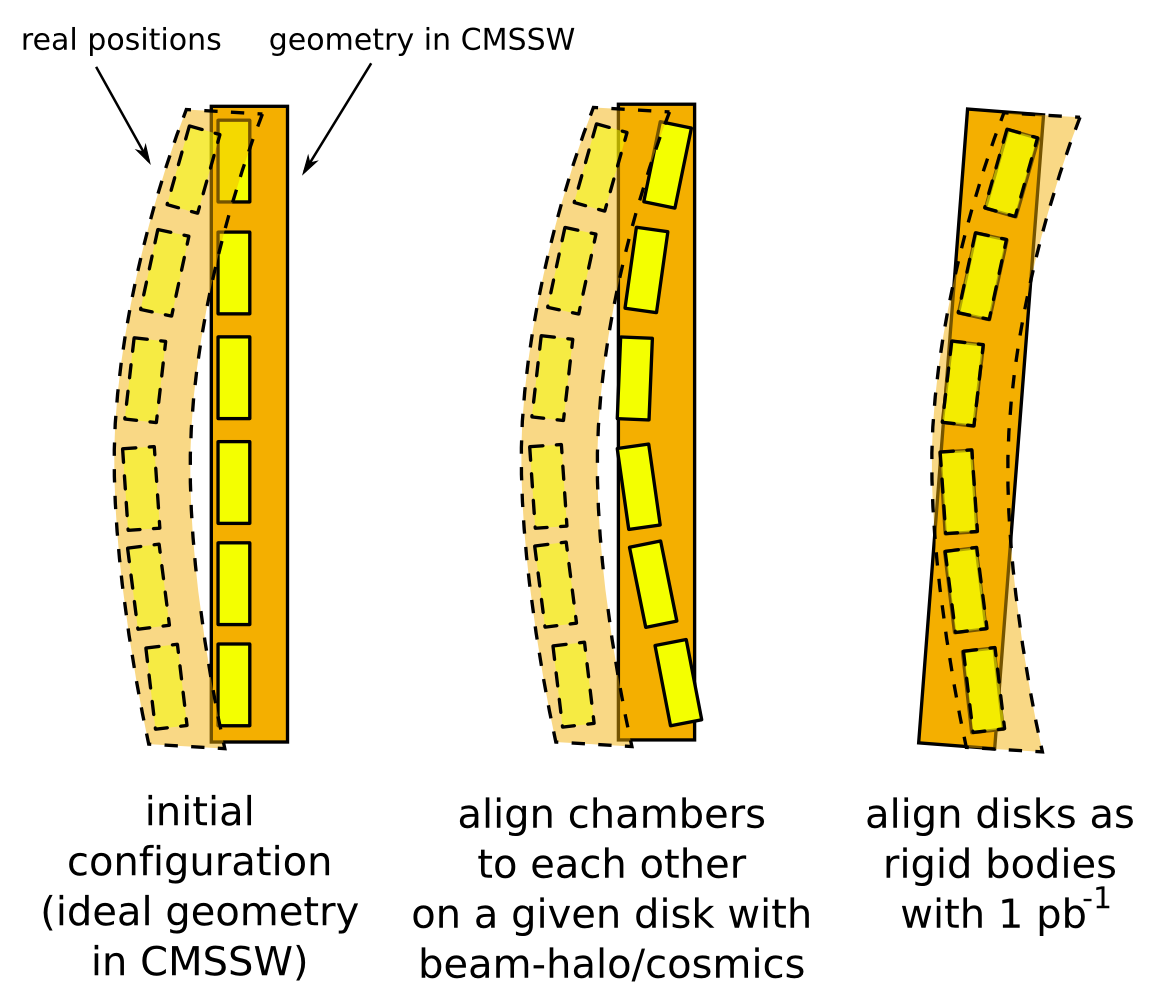
\includegraphics[width=0.9\linewidth]{plan.png} \end{center}
\end{frame}

\begin{frame}
\frametitle{Role of beam-halo/cosmics}
\textcolor{darkblue}{Goal A-1:} align chambers ($x$, $y$, $\phi_y$, $\phi_z$) in each station
\begin{itemize}
\item requires beam-halo in the overlap regions (no ME1/3)
\item track propagation is short and avoids iron; beam-halo orientation is perfect
\item whole-station parameters are unconstrained (the whole station
can rotate, and that's okay)
\end{itemize}

\vfill
\textcolor{darkblue}{Goal A-2:} align chambers ($x$, $y$, $z$, $\phi_x$?, $\phi_y$, $\phi_z$) on each disk
\begin{itemize}
\item (alternative to \textcolor{darkblue}{A-1})
\item additionally requires cosmic rays to access $z$ and $\phi_x$ and to connect
chambers in different rings
\item track propagation still avoids iron
\item whole-disk parameters are unconstrained (that's okay)
\end{itemize}

\vfill
\textcolor{darkblue}{Goal B:} align layers ($x$, $y$, $\phi_y$, $\phi_z$) in each chamber
\begin{itemize}
\item requires overlap beam-halo with large statistics (no ME1/3)
\item constrain whole-chamber parameters by combining with
\textcolor{darkblue}{A-1} or \textcolor{darkblue}{A-2} (above)
\end{itemize}
\end{frame}

\begin{frame}
\frametitle{Procedure for goal A-1:}
Split station by even- and odd-numbered chambers

\vspace{-0.25 cm}
\begin{center} 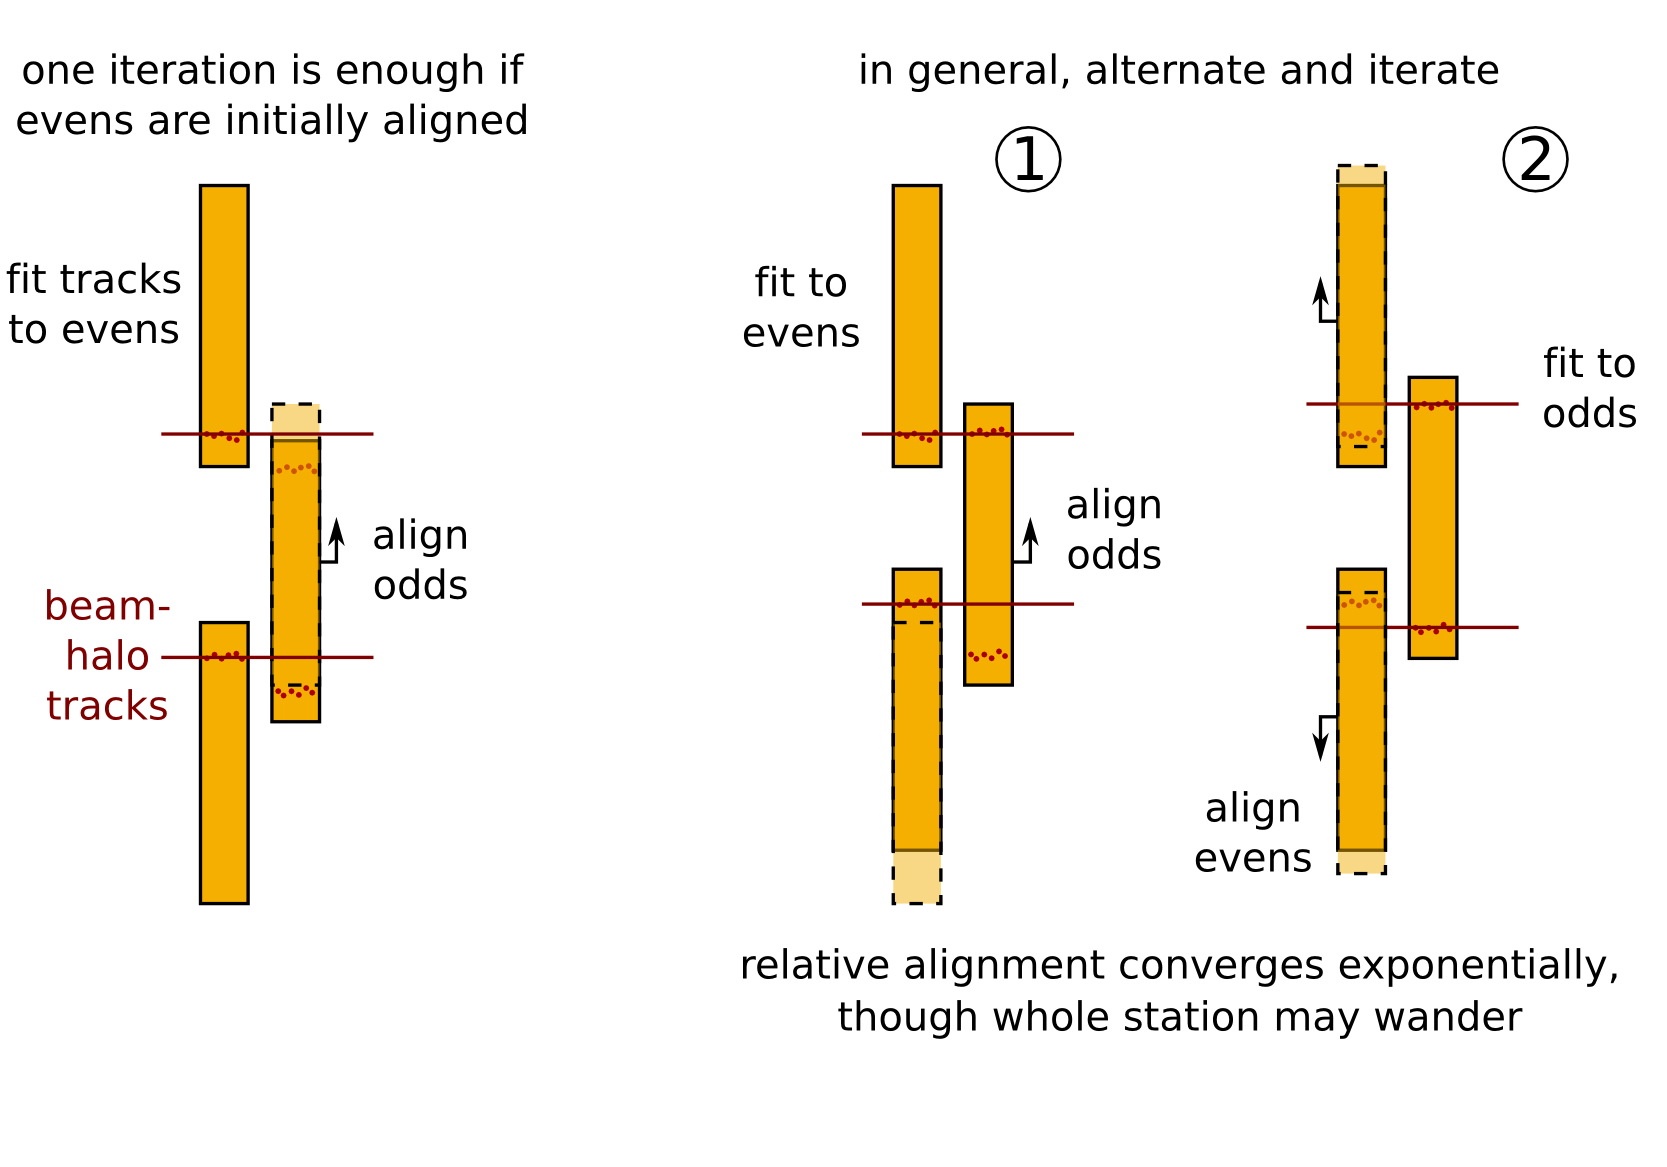
\includegraphics[width=0.9\linewidth]{illustration-A1.png} \end{center}

\vspace{-1 cm}
\begin{itemize}
\item Overlap hits are now included on tracks (Rick Wilkinson)
\item Need to set APEs of even-numbered chambers in chosen station to 0, all others to $\infty$
\end{itemize}
\end{frame}

\begin{frame}
\frametitle{Extend procedure to cover goal B?}
\begin{center} 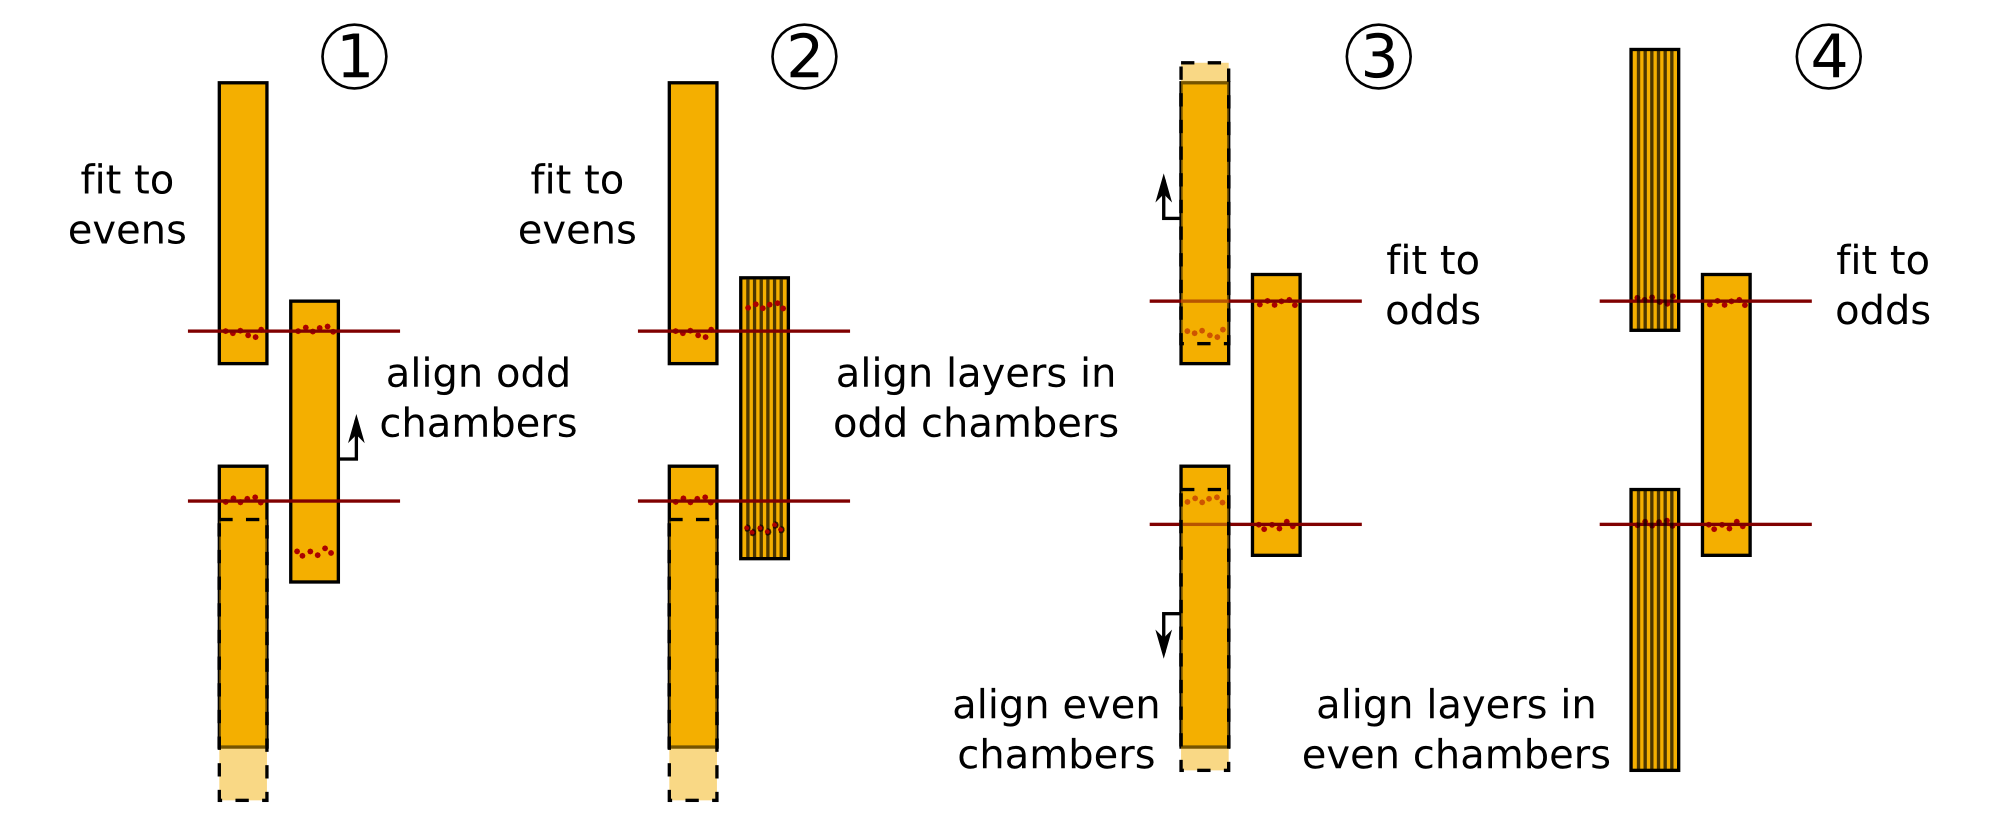
\includegraphics[width=\linewidth]{illustration-B.png} \end{center}

\begin{itemize}
\item Add another step for layer alignment, after centering chamber position
\item Requires higher statistics because we now have 1 hit per alignable per track, rather than 6
\end{itemize}
\end{frame}

\begin{frame}
\frametitle{Even/odd structure of the muon system}
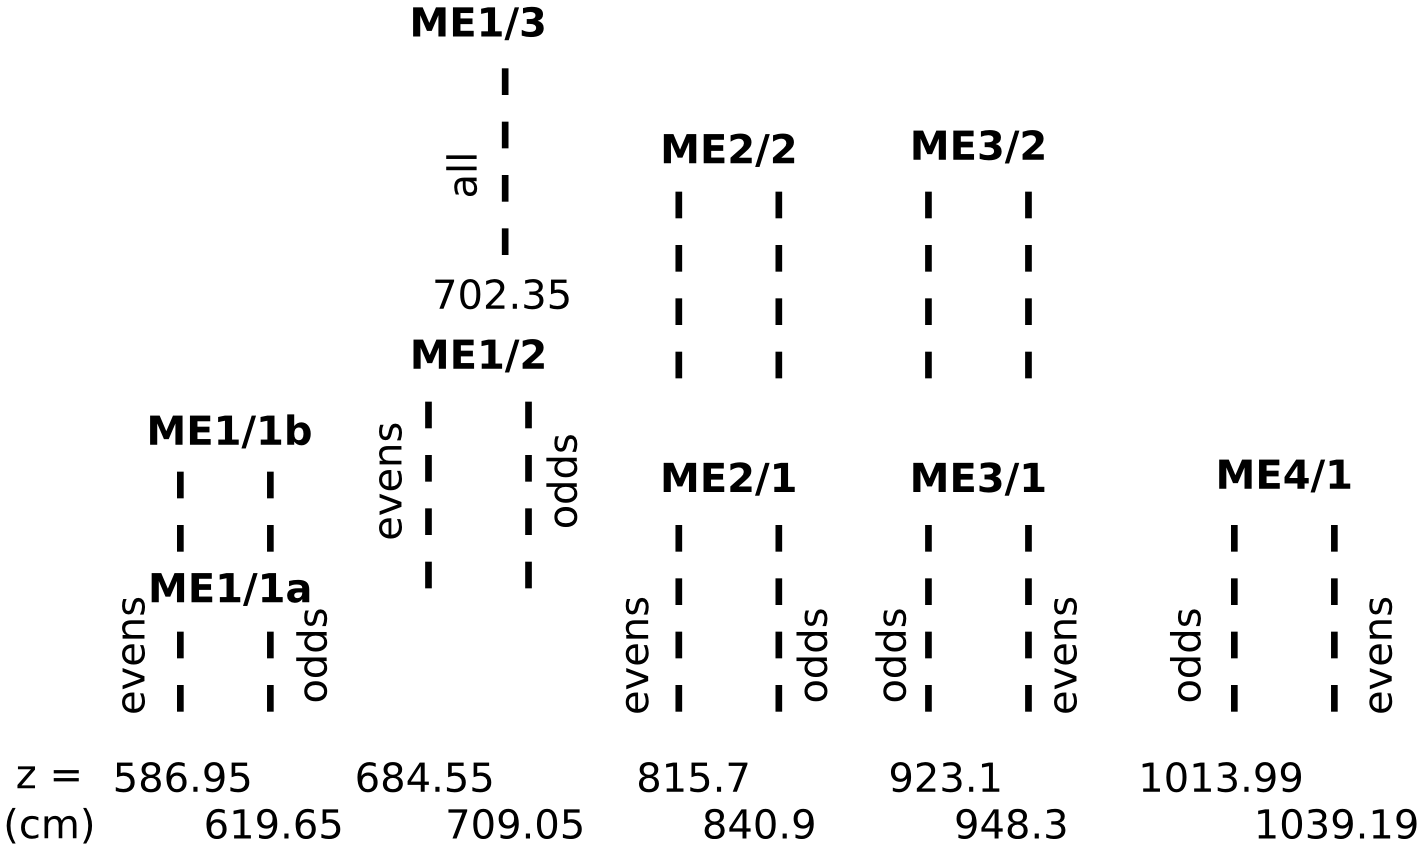
\includegraphics[width=\linewidth]{evenodd.png}
\begin{itemize}
\item Cosmic rays could connect ring 2 even with ring 1 odd
\item All ME1/3 chambers must be treated as ``odds''
\item No way to connect ME1/1 with ME1/2, 1/3
\end{itemize}
\end{frame}

\begin{frame}
\frametitle{Extend procedure to cover goal A-2?}
\vspace{-0.25 cm}
\begin{itemize}
\item Mix cosmic rays with beam-gas and group sets of chambers appropriately
\end{itemize}

\vspace{0.25 cm}
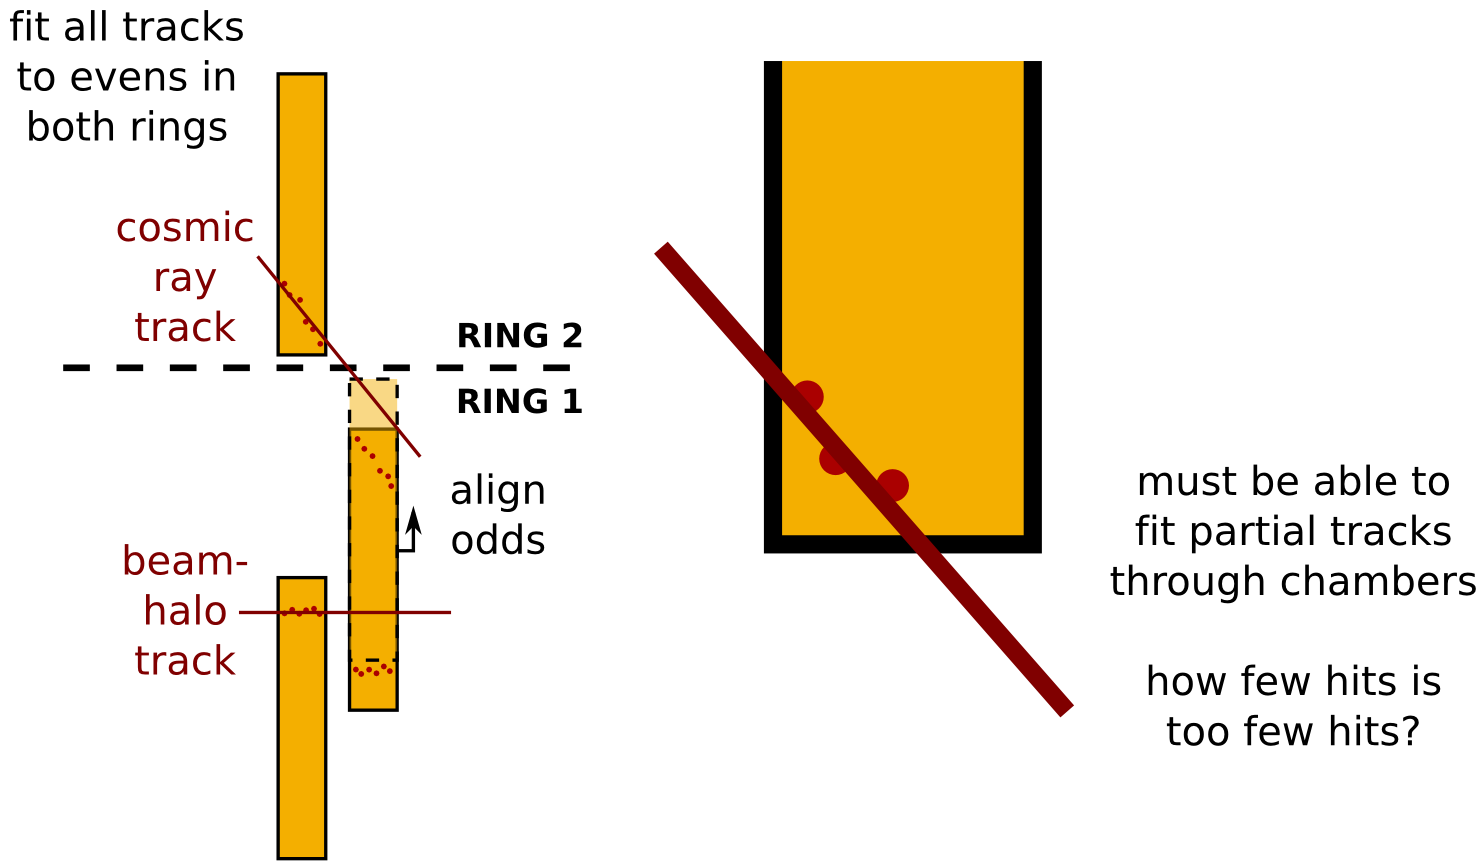
\includegraphics[width=\linewidth]{illustration-A2.png}
\end{frame}

\begin{frame}
\frametitle{Role of 1~pb$^{-1}$}
\begin{itemize}
\item Align whole-station or whole-disk structures to tracker coordinate system using globalMuons
\item Very few tracks (hundreds) are needed for full 6 d.o.f.
\item BUT\ldots Software infrastructure can only align whole disks, where ME1/1a, ME1/1b, ME1/2, and ME1/3 are one disk
\begin{itemize}
\item If goal A-2 is achieved, we still wouldn't be able to align ME1/1 relative to ME1/2-ME1/3 structure
\item If goal A-2 is unattainable, we would need to rely on 1~pb$^{-1}$ for relative alignment of stations on a disk
\end{itemize}
\item This is a rather significant modification to the code--- unclear
if I can do this by 2\_0\_0 and it's late to ask
\end{itemize}

\vfill
\hspace{-0.83 cm} \textcolor{darkblue}{\Large Potential role of hardware alignment}
\begin{itemize}
\item Straight-line monitors were designed to connect inner ring with outer ring ($z$ deformation)
\item I don't know of any connection between ME1/1 and ME1/2-ME1/3
\end{itemize}

\label{numpages}
\end{frame}

\end{document}
